\documentclass[14pt, a4paper]{article}
\usepackage[utf8]{inputenc}
\usepackage[russian]{babel}
\usepackage{graphicx}

\title{\textbf{Отчет о выполнении лабораторной работы 1.1.1}}
\author{Калашников Михаил, Б03-205}
\date{}

\begin{document}

\maketitle

В работе используются линейка, штангенциркуль, микрометр, отрезок из проволоки из нихрома, амперметр, вольтметр, источник ЭДС, мост постоянного тока,  реостат, ключ.

\begin{enumerate}

\item Точность измерения с помощью штангенциркуля -- $0.1\ mm$. Точность измерения с помощью микрометра -- $0.01\ mm$.

\item Измеряем диаметр проволоки штангенциркулем ($d_1$) и микрометром ($d_2$) на 10 различных участках (табл. \ref{table1}).

\[\bar{d_1}=0.4\ mm,\ \bar{d_2}=0.363\ mm\]

\begin{table}[!h]
\centering
\begin{tabular}{| c | c | c | c | c | c | c | c | c | c | c |}
\hline
& 1 & 2 & 3 & 4 & 5 & 6 & 7 & 8 & 9 & 10 \\
\hline
$d_1, mm$ & 0.4 & 0.4 & 0.4 & 0.4 & 0.4 & 0.4 & 0.4 & 0.4 & 0.4 & 0.4 \\
\hline
$d_2, mm$ & 0.36 & 0.36 & 0.36 & 0.36 & 0.36 & 0.36 & 0.36 & 0.37 & 0.37 & 0.37 \\
\hline
& \multicolumn{10}{c |}{\scriptsize{$\bar{d_1}=0.4\ mm\ \ \ \ \bar{d_2}=0.363\ mm$}} \\
\hline
\end{tabular}
\caption{Результаты измерения диаметра проволоки}
\label{table1}
\end{table}

При измерении диаметра проволоки штангенциркулем случайная погрешность измерения отсутствует. Следовательно, точность результата определяется только точностью штангенциркуля (систематической погрешностью):

\[d_1=(0.4\pm0.1)\ mm.\]

Измерения с помощью микрометра содержат как систематическую, так и случайную погрешности:

\[\sigma_{syst}=0.01\ mm,\ \sigma_{rand}=\frac{1}{N}\sqrt{\sum_{i=1}^{N}\left(d_2-\bar{d}\right)^2}=\frac{1}{10}\sqrt{2.1\cdot10^{-4}}\approx1.4\cdot10^{-3}\ mm,\]

\[\sigma_d=\sqrt{\sigma_{syst}^2+\sigma_{rand}^2}=\sqrt{(0.01)^2+(0.0014)^2}\approx0.01\ mm.\]

Поскольку $\sigma_{rand}^2\ll\sigma_{syst}^2$, то можно считать проволоку однородной по диаметру, а погрешность диаметра $\sigma_d$ определяется только $\sigma_{syst}$ микрометра:

\[d_2=\bar{d_2}\pm\sigma_d=(0.363\pm0.010)\ mm=(3.63\pm0.10)\cdot10^{-2}\ cm.\]

\item Определим площадь поперечного сечения проволоки:

\[S=\frac{\pi d_2^2}{4}=\frac{3.14\cdot(3.63\cdot10^{-2})^2}{4}\approx1.03\cdot10^{-3}\ cm^2.\]

Величину погрешности $\sigma_s$ найдем по формуле

\[\sigma_s=2\frac{\sigma_d}{d}S=2\frac{0.01}{0.363}\cdot1.03\cdot10^{-3}\approx5.7\cdot10^{-5}\ cm^{2}.\]

Итак, $S=(1.03\pm0.057)\cdot10^{-3}\ cm^2$, т.е. площадь поперечного сечения проволоки определена с точностью 6\%.

\item Сведем основные характеристики приборов в табл. \ref{table2}.

\begin{table}[!h]
\centering
\begin{tabular}{| l | c | c |}
\hline
& Вольтметр & Амперметр \\
\hline
Система & Магнитоэлектрическая & Цифровая \\
Класс точности & 0.5 & 0.5 \\
Предел измерений $x_n$ & 0.75 V & 2 A\\
Число делений шкалы $n$ & 150 & - \\
Цена делений $\frac{x_n}{n}$ & 5 mV/дел & - \\
Чувствительность $\frac{n}{x_n}$ & 200 дел/V & - \\
Абсолютная погрешность $\Delta x_M$ & 2.5 mV & 0.3 mA \\
Внутреннее сопротивление прибора & 250 $\Omega$ & 1.2 $\Omega$ \\
\hline
\end{tabular}
\caption{Основные характеристики приборов}
\label{table2}
\end{table}

\item Известно, что $R_{pr}\approx5\ \Omega$, $R_V=250\ \Omega$, $R_A=1.2\ \Omega$. Оценим по формулам (4) и (5) величину поправок при измерении $R_{pr}$: \\
для схемы рис. \ref{image1}а $R_{pr}/R_V=5/250$, т.е. 2\%; \\
для схемы рис. \ref{image1}б $R_{A}/R_{pr}=1.2/5$, т.е. 24\%. \\
Вывод: при измерении относительно небольших сопротивлений меньшую ошибку дает схема \ref{image1}а.

\item Собираем схему \ref{image1}а.

\begin{figure}
\includegraphics[width=\linewidth]{circuts.png}
\caption{Схемы для измерения сопротивления при помощи амперметра и вольтметра}
\label{image1}
\end{figure}

\item Опыт проводим для следующих трех длин проволоки: \\
$l_1=(20.0\pm0.1)\ cm$; $l_2=(30.0\pm0.1)\ cm$; $l_3=(50.0\pm0.1)\ cm$. \\
Показания приборов записываем в табл. \ref{table3}. Результаты измерения сопротивлений с помощью моста заносим в табл. \ref{table4}.

\item Строим графики зависимостей $V=f(I)$ для всех трех отрезков проволоки, проводя прямые через экспериментальные точки (рис. \ref{image2}).

\item Для каждой длины $l$ расчет проводим методом наименьших квадратов для прямой, проходящей через начало координат. Сопротивление находим как $R_{av}=\frac{\langle VI \rangle}{\langle I^2 \rangle}$ и его среднеквадратичную случайную ошибку как $\sigma_{R_{av}}^{rand}=\frac{1}{\sqrt{N}}\sqrt{\frac{\langle V^2\rangle}{\langle I^2\rangle}-R_{av}^2}$, где N	-- число экспериментальных точек. Результаты запишем в табл. \ref{table4}.

\begin{figure}
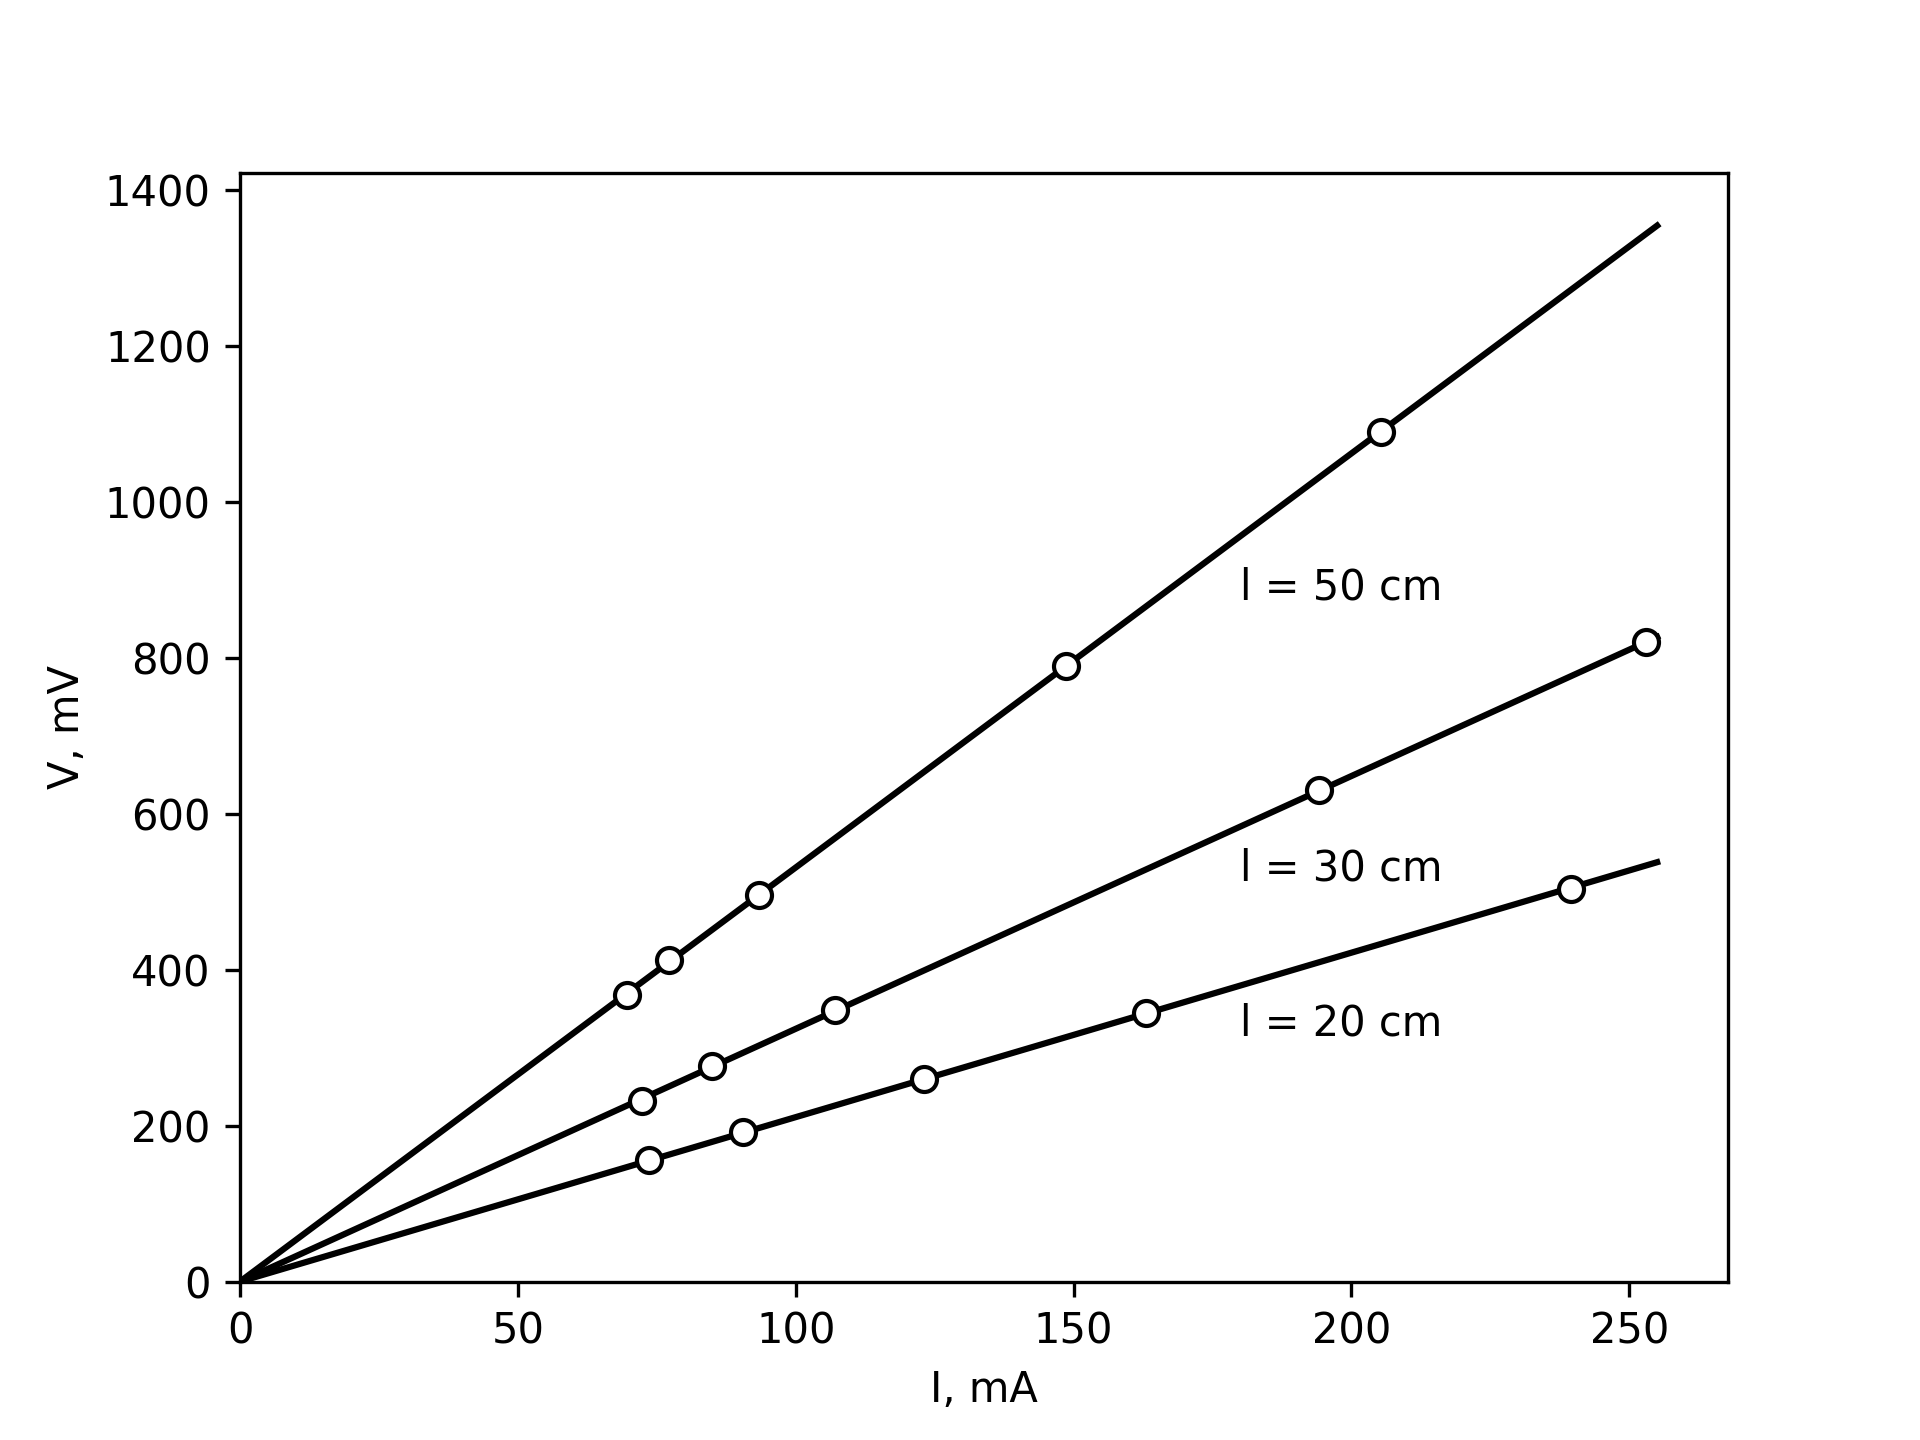
\includegraphics[width=\linewidth]{laba2.png}
\caption{График зависимости $V=f(I)$}
\label{image2}
\end{figure}

\begin{table}[!h]
\centering
\begin{tabular}{| c | c || c | c || c | c |}
\hline
\multicolumn{2}{| c ||}{$l=20\ cm$} & \multicolumn{2}{| c ||}{$l=30\ cm$}  & \multicolumn{2}{| c |}{$l=50\ cm$} \\
\hline
$V,$ & $I,$ & $V,$ & $I,$ & $V,$ & $I,$ \\
$mV$ & $mA$ & $mV$ & $mA$ & $mV$ & $mA$ \\
\hline
156 & 73.56 & 232 & 72.25 & 368 & 69.62 \\
192 & 90.49 & 276 & 85.0 & 412 & 77.22 \\
260 & 123.02 & 348 & 107.12 & 496 & 93.35 \\
344 & 163.05 & 630 & 194.12 & 790 & 148.6 \\
504 & 239.44 & 820 & 253.04 & 1090 & 205.4 \\
\hline
\end{tabular}
\caption{Показания вольтметра и амперметра}
\label{table3}
\end{table}

\begin{table}[!h]
\centering
\begin{tabular}{| c || c || c |}
\hline
$l=20\ cm$ & $l=30\ cm$ & $l=50\ cm$ \\
\hline
$R_0=2.120\ \Omega$ & $R_0=3.235\ \Omega$ & $R_0=5.312\ \Omega$ \\
$R_{av}=2.109\ \Omega$ & $R_{av}=3.242\ \Omega$ & $R_{av}=5.311\ \Omega$ \\
$R_{pr}=2.127\ \Omega$ & $R_{pr}=3.284\ \Omega$ & $R_{pr}=5.424\ \Omega$ \\
$\sigma_R^{rand}=0.002\ \Omega$ & $\sigma_R^{rand}=0.003\ \Omega$ & $\sigma_R^{rand}=0.004\ \Omega$ \\
$\sigma_R^{syst}=0.005\ \Omega$ & $\sigma_R^{syst}=0.005\ \Omega$ & $\sigma_R^{syst}=0.007\ \Omega$ \\
$\sigma_R=0.006\ \Omega$ & $\sigma_R=0.006\ \Omega$ & $\sigma_R=0.008\ \Omega$ \\
\hline
\end{tabular}
\caption{Результаты измерения сопротивления проволоки}
\label{table4}
\end{table}

\item Возможную систематическую погрешность $R_{av}$ оцениваем по формуле

\[\frac{\sigma_{R_{av}}^{syst}}{R_{av}}=\sqrt{\left(\frac{\sigma_V}{V}\right)^2+\left(\frac{\sigma_I}{I}\right)^2},\] 

где $I$ и $V$ -- максимальные значения тока и напряжения, полученные в эксперименте, а $\sigma_V$ и $\sigma_I$ -- ошибки измерения вольтметра и амперметром. Ошибка $\sigma_V$ равна половине абсолютной погрешности вольтметра:

\[\sigma_V=\frac{\Delta x}{2}=\frac{2.5}{2}\approx1.25\ mV.\]

Аналогично для амперметра:

\[\sigma_I=\frac{\Delta x}{2}=\frac{0.3}{2}\approx0.15\ mA.\]

Пример расчета $\sigma_{R_{av}}$ для проволоки длиной $l=30\ 	cm$; из табл. \ref{table3} и \ref{table4} $R_{av}=3.242\ \Omega$, $V=820\ mV$, $I=253.04\ mA$.

\[\sigma_{R_{av}}=R_{av}\sqrt{\left(\frac{\sigma_V}{V}\right)^2+\left(\frac{\sigma_I}{I}\right)^2}=3.242\cdot\sqrt{\left(\frac{1.25}{820}\right)^2+\left(\frac{0.15}{253.04}\right)^2}\approx5.3\cdot10^{-3}\ \Omega.\]

Складываем случайную и систематическую ошибки по формуле $\sigma_R=\sqrt{(\sigma_R^{rand})^2+(\sigma_R^{syst})^2}$  и результаты заносим в табл. \ref{table5}.

\begin{table}[!h]
\centering
\begin{tabular}{| c | c | c | c |}
\hline
$l, cm$ & 20 & 30 & 50 \\
\hline
$R_{av}, \Omega$ & 2.109 & 3.242 & 5.311 \\
\hline
$\sigma_R, \Omega$ & 0.006 & 0.006 & 0.008 \\
\hline
\end{tabular}
\caption{Значения $R_{av}$ и $\sigma_R$ для каждого значения $l$}
\label{table5}
\end{table}

\item Для всех трех длин $l$ вносим поправку в измеренное значение сопротивления по формуле

\[R_{pr}=R_{av}+\frac{R_{av}^2}{R_V}.\]

Ввиду малости поправки считаем $\sigma_{R_{pr}}=\sigma_{R_{av}}$. Данные заносим в табл. \ref{table4}.

\item Сравниваем результаты измерения сопротивления проволоки с помощью вольтметра и амперметра с результатами измерений мостом. В пределах погрешностей опыта результаты совпадают.

\item Определим удельное сопротивление проволоки по формуле

\[\rho=\frac{R_{pr}}{l}\frac{\pi d^2}{4}\]

и погрешность $\sigma_{\rho}$ по формуле

\[\frac{\sigma_{\rho}}{\rho}=\sqrt{\left(\frac{\sigma_R}{R}\right)^2+\left(2\frac{\sigma_d}{d}\right)^2+\left(\frac{\sigma_l}{l}\right)^2}\]

и заносим результаты в табл. \ref{table6}.

\begin{table}[!h]
\centering
\begin{tabular}{| c | c | c |}
\hline
$l, cm$ & $\rho,\ 10^{-4}\ \Omega\cdot cm$ & $\sigma_{\rho},\ 10^{-6}\ \Omega\cdot cm$ \\
\hline
20 & 1.10 & 6.1 \\
30 & 1.13 & 6.3 \\
50 & 1.12 & 6.2 \\
\hline
\end{tabular}
\caption{Значения $R_{av}$ и $\sigma_R$ для каждого значения $l$}
\label{table6}
\end{table}

\end{enumerate}

Окончательно: $\rho=(1.12\pm0.06)\cdot10^{-4}\ \Omega\cdot cm.$

\par

Основной вклад в ошибку $\sigma_{rho}$ вносит погрешность измерения диаметра проволоки, составляющая $\sim$3\%, но так как из-за возведения в квадрат она удваивается, вклад в погрешность удваивается, вклад в погрешность результата составляет $\sim$6\%. Поэтому при измерении сопротивления проволоки достаточна точность 3--4\%.

\par

Полученное значение удельного сопротивления сравниваем с табличными значениями. В справочнике (Физические величины. М.: Энергоиздат, 1991. С. 444) для удельного сопротивления нихрома при $20^{\circ}C$ значения в зависимости от массового содержания компонент сплава меняются от $0.97\cdot10^{-4}\ \Omega\cdot cm$ до $1.12\cdot10^{-4}\ \Omega\cdot cm$. Для получившегося в работе $1.12\cdot10^{-4}\ \Omega\cdot cm$ массовое содержание компонентов: 63\% Ni, 20\% Fe, 15\% Cr, 2\% Mn (проценты по массе).

\end{document}